\section{System Integration}
\label{sec:integration_implementation}

Complex robotics systems achieve their full potential only through seamless integration of their constituent subsystems. While individual components may function correctly in isolation, the coordination between hardware controllers, software nodes, perception algorithms, and external interfaces determines whether the system operates as a unified platform or remains a collection of disconnected modules. This chapter presents the integration methodology that transforms the Tino V2's diverse components into a cohesive VR-embodied robotic system capable of real-time social interaction.

The integration challenges extend beyond simple component interconnection. The system must coordinate multiple Arduino controllers operating at different speeds, synchronize perception data from various sensors, maintain real-time communication with VR systems, and ensure that atomic movement commands execute reliably despite network latencies and computational loads. Additionally, the integration must support both development workflows—where individual subsystems require isolated testing—and production deployment where all components operate simultaneously.

\subsection{System Architecture Integration}

The integration methodology addresses the fundamental challenge of coordinating diverse subsystems that operate across different computational platforms, communication protocols, and timing requirements. The solution employs a layered architecture where ROS2 serves as the central coordination layer, managing communication between hardware interfaces, perception modules, and external systems while maintaining modularity for development and debugging.

\subsubsection{ROS2 Node Orchestration}

The distributed ROS2 architecture enables sophisticated parallel processing while maintaining reliable inter-node communication through the Data Distribution Service middleware. The six primary nodes—gamepad control, hardware interface, robot controller, pose detection, VR interface, and UWB positioning—operate as independent processes that communicate through standardized message interfaces, enabling optimal utilization of the Orin Nano's multi-core architecture.

Node interdependencies follow a carefully designed communication graph that prevents circular dependencies while enabling rich data sharing. The robot controller node serves as the central coordination hub, receiving localization data from RTABMap, absolute positioning from UWB, and movement commands from either gamepad or VR interface nodes. This centralized approach enables sophisticated sensor fusion and behavior coordination while maintaining loose coupling between subsystems.

Launch file orchestration manages the complex startup sequence required for reliable system initialization. The \texttt{start\_tino\_with\_rtab.launch.py} configuration implements staged initialization where camera and IMU systems initialize first, followed by SLAM nodes, then hardware interfaces, and finally VR communication nodes. This sequencing prevents initialization race conditions while ensuring that critical dependencies like camera calibration and IMU orientation are established before dependent systems come online.

Quality of Service (QoS) policies optimize communication reliability for different data types: sensor data utilizes ``best effort'' delivery for maximum throughput, control commands employ ``reliable'' delivery to ensure execution, and system health monitoring uses ``transient local'' durability to maintain state information across node restarts. These differentiated QoS policies enable optimal performance while maintaining system reliability.

\subsubsection{Hardware-Software Interface Coordination}

The integration between software control systems and physical hardware requires sophisticated coordination to handle the disparate timing characteristics of Arduino controllers, ROS2 nodes, and VR systems. The hardware interface node implements thread-based communication management that maintains independent serial connections to three Arduino controllers while coordinating their combined operation through centralized command generation.

\begin{figure}[H]
    \centering
    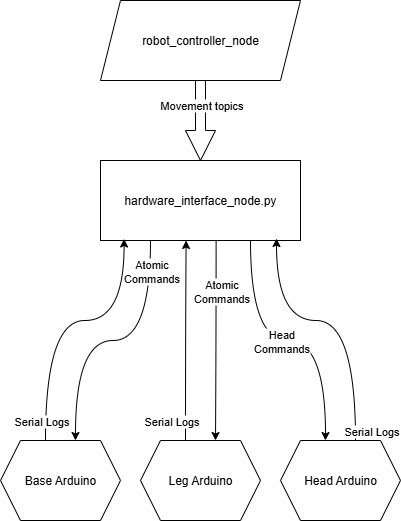
\includegraphics[height=6cm]{Images/HardwareNodeInteraction.png}
    \caption{Hardware Interface Node Communication Architecture}
    \label{fig:hardware_node_interaction}
\end{figure}

Serial communication reliability employs several integration strategies to ensure robust operation. Persistent device naming through udev rules (\texttt{/dev/ttyBASE}, \texttt{/dev/ttyLEG}, \texttt{/dev/ttyHEAD}) eliminates device enumeration variability that could disrupt system startup. Triple-redundant command transmission at the protocol level ensures message delivery across communication disruptions, while thread-based connection monitoring enables automatic reconnection without affecting other subsystem operations.

The atomic movement coordination system demonstrates sophisticated integration between software control logic and hardware execution timing. State transitions must coordinate between leg extensions (requiring encoder feedback) and base movements (using timer-based control) while handling the different response characteristics of each subsystem. The integration ensures that compound movements like ``extend leg, move base, retract leg'' execute as atomic operations despite involving multiple physical controllers with independent timing requirements.

Command format standardization through the key-value protocol (\texttt{BF=value,BB=value,HP=value,HX=value,HY=value}) enables unified control message generation while accommodating the different parameter requirements of each controller. This integration approach maintains backward compatibility with existing Arduino firmware while enabling sophisticated coordination through the ROS2 layer.

\subsection{Perception-Control Integration}

Real-time VR teleoperation requires seamless integration between perception systems that understand the environment and control systems that execute user commands. The integration addresses fundamental challenges in coordinate frame alignment, temporal synchronization, and data fusion that enable natural VR interaction with reliable environmental awareness.

\subsubsection{Sensor Fusion Coordination}

The integration coordinates complementary sensing modalities through the robot controller node, which implements position-orientation decomposition to leverage UWB absolute positioning alongside RTABMap visual orientation. This hybrid approach addresses the fundamental challenge of maintaining accurate localization while supporting real-time VR interaction requirements.

The integration handles coordinate frame alignment through systematic transformation and implements graceful degradation when individual sensors become unavailable. The resulting fused pose data provides VR operators with reliable spatial reference for immersive teleoperation, demonstrating how multiple perception systems can be effectively coordinated through centralized sensor fusion architecture.

\subsubsection{Human Detection and Spatial Awareness}

The integration of human pose detection with the VR interface provides essential environmental awareness for remote operators. The system coordinates YOLOv11 pose estimation with stereo depth processing to deliver comprehensive human positioning data to Unity VR environments, enabling informed decision-making during teleoperated social interaction.

The integration transforms 2D pose detections into 3D spatial information through depth-pose fusion, then packages this data into standardized 208-byte UDP packets for VR consumption. This perception-to-VR pipeline ensures that remote operators maintain situational awareness of human presence and positioning, critical for effective social robotics research through immersive teleoperation.

\subsection{VR Communication Integration}

The VR interface integration addresses the complex challenge of maintaining real-time bidirectional communication between Unity VR environments and the robot control system. The integration must handle network latency variability, command ordering, and data synchronization while maintaining the responsiveness required for natural teleoperation.

\subsubsection{UDP Protocol Optimization}

The VR integration employs custom UDP protocols designed specifically for real-time robot teleoperation requirements. The three-port architecture isolates command streams from data streams, enabling optimized communication patterns that maintain sub-10ms latency while providing reliable command delivery.

The integration addresses the fundamental challenge of bridging Unity's game engine architecture with ROS2's middleware through protocol optimization and message ordering validation. This approach achieves the responsiveness required for natural VR interaction while maintaining sufficient reliability for production robot operation.

\subsubsection{Unity-ROS2 Bridge Architecture}

The VR integration bridges Unity's game engine with ROS2's robotic middleware through coordinated data transformation and communication management. The system handles coordinate system alignment, real-time data formatting, and bidirectional audio integration to enable natural VR teleoperation of the robot platform.

This integration demonstrates how game engine architectures can be effectively coupled with robotic control systems through protocol optimization and data format standardization, enabling immersive teleoperation while maintaining the modularity of the underlying robot architecture.

\subsection{Launch File and System Orchestration}

System deployment requires sophisticated orchestration that coordinates the startup sequence, parameter management, and runtime monitoring of multiple interconnected nodes. The integration employs structured launch files and tmux session management to provide reliable system deployment while supporting development workflows.

\subsubsection{Parameterized Launch Configuration}

Launch file integration addresses the challenge of managing dozens of configuration parameters across multiple nodes while maintaining flexibility for different operational modes. The main launch configuration (\texttt{start\_tino\_with\_rtab.launch.py}) implements hierarchical parameter management where device-specific settings like serial ports and camera configurations cascade through node-specific launch files.

Device persistence integration through udev rules ensures consistent hardware mapping across system restarts. The \texttt{99-tino-arduino.rules} configuration creates persistent symlinks that eliminate device enumeration variability, enabling reliable hardware interface initialization regardless of USB connection order or system hardware changes.

Conditional node launching supports both development and production deployment modes. The gamepad node activation depends on hardware availability detection, while VR interface nodes can operate in simulation mode when Unity systems are unavailable. This integration flexibility enables comprehensive testing and gradual system deployment.

\subsubsection{Runtime Monitoring and Recovery}

Health monitoring integration provides comprehensive system state awareness while enabling automatic recovery from common failure modes. The robot controller node implements sophisticated monitoring that tracks RTABMap operation health, UWB communication status, and hardware interface connectivity.

Automatic recovery procedures demonstrate integration-level resilience design. RTABMap orientation loss triggers odometry reset sequences through the \texttt{/reset\_odom} service, while UWB communication failures activate graceful fallback to visual odometry only. Hardware interface reconnection procedures operate independently for each Arduino controller, maintaining partial system operation during individual hardware failures.

Tmux session management provides integrated process coordination that supports both operational deployment and development debugging. The session structure separates RTABMap visualization (left pane) from robot control logging (right pane), enabling simultaneous monitoring of mapping performance and control system operation. Session persistence across SSH disconnections ensures continuous operation during remote development and deployment.

The successful integration transforms individual hardware and software components into a unified VR-embodied robotic platform. The ROS2-based coordination layer enables seamless communication between perception systems, control algorithms, and VR interfaces while maintaining the modularity essential for continued development. This integration architecture demonstrates how sophisticated robotic capabilities can be effectively orchestrated through well-designed middleware approaches, creating a foundation for advanced social robotics research through immersive virtual reality teleoperation.
